% Fig. 3.8 -- 兩個變數比大小所對應的區域: 直線 x_1 = x_2 的左上方。
% 書稿來源: mathstatch3.tex 第 931 行的 tikzpicture。
%
% 書稿此圖排在解答文字右側的 minipage 之內，網頁改置於文字下方。
% 幾何一律照書稿: 由原點畫到 (1,1) 的斜線、其左上方的三角形填色、
% 由 (1,1) 各拉一條虛線到兩軸並各標 1、兩軸帶箭頭並標 x_1 與 x_2。
%
% 對書稿的兩處調整:
%   1. 填色由 gray 0.2 改為 journalaccent 0.15，兩條界線改 journalmuted 虛線。
%   2. 書稿把 $x_1$ 標在 (3.5,0.15)、$x_2$ 標在 (0,3.8)，都離軸端有一段距離；
%      本圖依 CH2 規格把軸名收到箭頭端點旁。
%   3. 字級與圖寬取與同一題的 Fig. 3.9、Fig. 3.10 一致 (10pt 內文、9pt 下標，
%      viewBox 寬同為 216.7pt)，三張圖並列時圖上的字一樣大。
%
% 檔名沿用 CH3_FIGURE_SPECS.md 所定的 independent-normal-region，先不改名。
%
% 量測: viewBox 寬 216.582pt，本圖置於 Example 方框之內，手機顯示寬 309px，
%       放大 1.4267 倍，最小字 9pt 折合 12.84px (350px 之下為 14.54px)。
%
% 產製:
%   pdflatex independent-normal-region.tex
%   pdftocairo -svg independent-normal-region.pdf ../../images/teaching-topics/independent-normal-region.svg

\documentclass[tikz,border=2pt]{standalone}
\usepackage{amsmath}
\usepackage{amssymb}
\usepackage{xcolor}

\definecolor{journalink}{HTML}{1F1C18}
\definecolor{journalmuted}{HTML}{8A7F72}
\definecolor{journalaccent}{HTML}{9C2D2D}

%% 10pt 之下的 script 級撐到 9pt，使兩軸軸名的下標夠大。
\DeclareMathSizes{10}{10}{9}{8}

\begin{document}
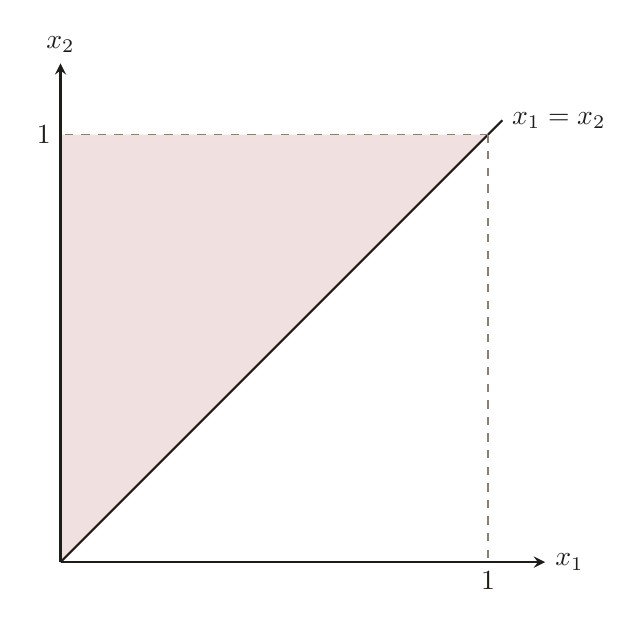
\begin{tikzpicture}[x=1.81cm, y=1.81cm, >=stealth,
                    every node/.style={journalink, font=\normalsize}]

  %% 所求範圍 x_1 < x_2: 直線 x_1 = x_2 的左上方
  \fill[journalaccent, fill opacity=0.15] (0,0) -- (3,3) -- (0,3) -- cycle;

  %% 邊界 x_1 = x_2
  \draw[journalink, line width=0.8pt] (0,0) -- (3.1,3.1);
  \node[journalink, right] at (3.1,3.1) {$x_1=x_2$};

  %% 值域的上界與右界
  \draw[journalmuted, line width=0.5pt, dashed] (3,3) -- (0,3);
  \draw[journalmuted, line width=0.5pt, dashed] (3,3) -- (3,0);
  \node[journalink, left]  at (0,3) {$1$};
  \node[journalink, below] at (3,0) {$1$};

  %% 座標軸
  \draw[journalink, line width=0.8pt, ->] (0,0) -- (3.4,0) node[right] {$x_1$};
  \draw[journalink, line width=0.8pt, ->] (0,0) -- (0,3.5) node[above] {$x_2$};

\end{tikzpicture}
\end{document}
